\section{Influence of temperature on the response of a straight pipe}
\subsection{Meaning and significance of stress terms}
\subsubsection{Principal stress}
\url{https://www.continuummechanics.org/principalstress.html}
Principal stress is a measure which defines the maximum normal stress which may be applied to a body of interest and where that stress is located. %Principal stress acts on the principal plane (an oblique plane at some angle $\theta$) and has the condition that there is zero shear stress on this plane. The resultant normal stresses acting on the principal plane, $\sigma_n$, is the principal stress. The normal stress can take a maximum or minimum value.
In the 3D case, we find that there exist three principal planes (where the shear stress is zero), which are orthogonal and each have their own maximum / minimum normal stresses. From this, we can also find locations and magnitude for the maximum shear stress.

Consider the six components of the 3D solid stress tensor:
\begin{equation}
    \sigma_{ij} = \begin{bmatrix}
        \sigma_x  & \tau_{yx} & \tau_{zx} \\
        \tau_{xy} & \sigma_y  & \tau_{zy} \\
        \tau_{xz} & \tau_{yz} & \sigma_z
    \end{bmatrix}
\end{equation}
where the first subscript denotes the direction of the surface normal and the second the direction of the stress. For static equilibrium:
\begin{equation}
    \tau_{xy} = \tau_{yx} \qquad \tau_{xz} = \tau_{zx} \qquad \tau_{zy} = \tau_{yz}
\end{equation}
By rotating the coordinate axes of our 3D body, we can change the components of the solid stress tensor, whilst representing the same state of stress on the body. As our matrix is symmetric, we can calculate a set of orthogonal axes which result in all $\tau$ elements equalling zero. This set of axes is called the principal axes and by applying this transformation to our solid stress tensor, we find the eigenvalues of the matrix and the principal stresses. Hence:
\begin{gather}
    \boldsymbol{\sigma}_{ij} = \begin{bmatrix}
        \sigma_x  & \tau_{yx} & \tau_{zx} \\
        \tau_{xy} & \sigma_y  & \tau_{zy} \\
        \tau_{xz} & \tau_{yz} & \sigma_z
    \end{bmatrix} \xrightarrow{eigenvalues} \boldsymbol{\sigma}_{ij}' = \begin{bmatrix}
        \sigma_1 & 0        & 0        \\
        0        & \sigma_2 & 0        \\
        0        & 0        & \sigma_3
    \end{bmatrix}\\
    \det(\boldsymbol{\sigma} - \sigma \boldsymbol{I}) = 0
\end{gather}
where $\boldsymbol{I}$ is the identity matrix and $\sigma$ is the eigenvalue. The eigenvectors of the stress tensor, which correspond to the principal directions (the angles between the original (or base) coordinate axes and the new (or transformed) coordinate axes), can be found by solving the equation:
\begin{equation}
    (\boldsymbol{\sigma} - \sigma \boldsymbol{I})\boldsymbol{v} = \boldsymbol{0}
\end{equation}
where $\boldsymbol{v}$ is the eigenvector. This may also be written as:
\begin{align}
    \cos \alpha = \cos\left(n, \, x\right) & = l \\
    \cos \beta = \cos\left(n, \, y\right)  & = m \\
    \cos \gamma = \cos\left(n, \, z\right) & = n
\end{align}
where $n$ is the unit normal to the plane. We can now define the normal stress acting on any oblique plane:
\begin{equation}
    \sigma_{x'} = \sigma_xl^2 + \sigma_y m^2 +\sigma_zn^2 + 2\left(\tau_{xy}lm + \tau_{xy}mn + \tau_{xz}ln\right)
\end{equation}
We are interested in the maximum and / or minimum values of the normal stress acting on our body throughout the range of oblique planes. These maxima / minima are the principal stresses. This is determined by calculating the differentials of the above equations with respect to the direction cosines. We find that the principal stresses occur on planes where the shear stress is zero, as mentioned previously. The equations for in-plane principal stresses are shown below. The third stress is zero in plane stress conditions.
\begin{gather}
    \sigma_1 = \left(\frac{\sigma_x + \sigma_y}{2}\right)+ \sqrt{\left(\frac{\sigma_x - \sigma_y}{2} \right)^2+ \tau^2_{xy} }\\
    \sigma_2 = \left(\frac{\sigma_x + \sigma_y}{2}\right)- \sqrt{\left(\frac{\sigma_x - \sigma_y}{2} \right)^2+ \tau^2_{xy} }
\end{gather}

A key characterisation of the principal stress is that it acts in the normal direction to the principal plane - this is important to note as a distinction. The determination of the principal stresses (and maximum shear stress) is important for design purposes as it tells us whether a body would be able to withstand a design load at a given location.
\subsubsection{Von Mises stress}
\url{https://www.continuummechanics.org/vonmisesstress.html}

Von Mises stress can be used to determine whether an isotropic and ductile material will yield under a complex loading condition. The von Mises stress equation is based on the principle that the failure of a material is dependent on the total amount of energy that is being absorbed by the material, rather than the individual stresses in each direction. The equation simplifies the complex stress state of a material, which is often composed of multiple stresses acting in different directions, into a single numerical value that is used to determine whether the material is likely to fail. A comparison between the material's yield stress and the von Mises stress allows the calculation of the von Mises Stress Criterion.

An equation for the von Mises stress is shown below.
\begin{equation}
    \sigma_{VM} = \sqrt{\frac{1}{2}\left[\left(\sigma_{x}-\sigma_y\right)^2 + \left(\sigma_y - \sigma_z\right)^2+\left(\sigma_z - \sigma_x\right)^2\right] + 3\left(\tau^2_{xy} + \tau^2_{yz}+\tau_{zx}^2\right)}
\end{equation}
However, we can also calculate the von Mises stress directly from the principal stresses (note that we may not do the reverse).
\begin{equation}
    \sigma_{VM} = \sqrt{\frac{1}{2}\left[\left(\sigma_1 - \sigma_2\right)^2 +\left(\sigma_2 - \sigma_3\right)^2 + \left(\sigma_3 - \sigma_1\right)^2 \right]}
\end{equation}

The von Mises stress is often used in engineering design to determine whether a material will fail under a given load. If the von Mises stress exceeds the yield strength of the material, plastic deformation is expected to occur. Therefore, designers can use the von Mises stress to ensure that their designs remain within the elastic limit of the material.
\subsubsection{Stress magnitude}
\subsection{Relationship between axial stress and temperature of length constrained 3D pipe}\label{part1b}
For a 3D pipe constrained against an increase in length (longitudinal strain being zero), we can draw the following schematic.

INSERT GRAPHIC

The derivation presented here concerns the thermal bowing of a laterally restrained beam or pipe subjected to a uniform temperature gradient. The derivation aims to obtain an equation that describes the lateral displacement of the beam due to the thermal load.

The starting point of the derivation is the expression for the displacement of a point in the beam. The displacement can be expressed as a function of the position along the beam, $x$, and two lateral coordinates, $y$ and $z$, as:
\begin{equation}
    u(x,y,z) = f(x) + yf_1(x) + zf_2(x)
\end{equation}
where $f(x)$ is the longitudinal displacement, $f_1(x)$ is the lateral slope, and $f_2(x)$ is the curvature.

The longitudinal strain in the beam can be expressed as the partial derivative of the displacement with respect to the longitudinal coordinate, $x$, as:
\begin{equation}
    \epsilon_{xx} = \frac{\partial u}{\partial x} = f'(x) + yf_1'(x) + zf_2'(x)
\end{equation}
The stress field in the beam can be expressed as a function of the longitudinal strain and the temperature distribution in the beam. Assuming that the temperature distribution is uniform and the longitudinal strain is solely due to thermal expansion, the stress field can be expressed as:
\begin{equation}
    \sigma_{xx} = E \left(\epsilon_{xx} - \alpha T\right)
\end{equation}
where $E$ is the modulus of elasticity of the material, $\alpha$ is the coefficient of thermal expansion, and $T$ is the temperature in the beam.

The equilibrium of forces and moments in the beam requires that the stress field integrates to zero over the cross-sectional area of the beam. Assuming that the temperature distribution is uniform, this condition can be expressed as:
\begin{align}
    \int \sigma_{xx} \dif A   & = 0 \\
    \int \sigma_{xx} y \dif A & = 0 \\
    \int \sigma_{xx} z \dif A & = 0
\end{align}
where $\dif A$ is an element of the cross-sectional area of the beam, and $y$ and $z$ are the lateral coordinates of the element.

The geometrical constraint is that the center of gravity of the cross-pipe must be located at the origin:
\begin{equation}
    \int y \dif A = \int z \dif A = 0
\end{equation}
Next, we consider the cross-pipe variation of temperature. The stress field in x-direction can be expressed as:
\begin{equation}
    \sigma_{xx} = -\alpha E\left(T - \bar{T}\right) + \frac{I_yM_{Tz}-I_{yx}M_{Ty}}{I_yI_z-I^2_{yz}}y + \frac{I_yM_{Tz}-I_{yx}M_{Ty}}{I_yI_z-I^2_{yz}}z
\end{equation}
where $T$ is the temperature at any given point, and $\bar{T}$ is the average temperature of the pipe. $I_z$, $I_y$ and $I_{yz}$ are the moments of inertia of the cross-sectional area with respect to yz, zx and xy planes respectively. $M_{Ty}$ and $M_{Tz}$ are the moments due to the variation of temperature.

For a pipe with a circular cross-section, $I_z$ and $I_y$ are equal, and $I_{yz}$ is zero. Hence, the stress field in the x-direction reduces to:
\begin{equation}
    \sigma_{xx} = -\alpha E \left(T - \bar{T}\right) + \frac{M_{Tz}}{I_y}y
\end{equation}
We can now derive the equation for lateral displacement of the pipe. The lateral displacement is obtained by taking the second derivative of the displacement function with respect to $x$:
\begin{gather}
    \frac{\dif^2 v}{\dif x^2} = - \frac{M_{Tz}}{EI_z}\\
    \frac{\dif}{\dif x^2}\left(EI_z\frac{\dif^2 v}{\dif x^2}\right) + \frac{\dif^2 M_{Tz}}{\dif x^2} = F
\end{gather}
The tensile force $P$ and a tensile $P-\delta$ moment $Py$ over the length of the beam give us the equation governing the displacement of the beam:
\begin{equation}
    \frac{\dif^2 y}{\dif x^2} = \phi + \frac{Py}{EI}
\end{equation}
where $y(x)$ is the displacement of the beam at position $x$, $\phi$ is the lateral displacement due to the uniform thermal gradient, $E$ is the Young's modulus, $I$ is the second moment of area.

Using the expression for the moment, $M = EI \phi = EI\alpha T_{,y}$, where $\alpha$ is the coefficient of thermal expansion and $T_{,y}$ is the temperature gradient, we can obtain the value of $P$ as:
\begin{equation}
    P = \frac{EI\alpha T_{,y}}{y}
\end{equation}
Substituting this expression for $P$ into the equation for the displacement, we get:
\begin{equation}
    \frac{\dif^2 y}{\dif x^2} - k^2 y = \phi
\end{equation}
where $k = \sqrt{P/EI}$. The solution to this differential equation is given by:
\begin{equation}
    y(x) = -\frac{\phi}{k^2}\left(\frac{\cosh(kl) - 1}{\sinh(kl)}\sinh(kx)\cosh(kx)+1\right)
\end{equation}
where $l$ is the length of the beam. This equation gives the displacement of the beam at any point $x$ due to the uniform thermal gradient, and it shows that the maximum displacement occurs at the mid-span of the beam, where
\begin{equation}
    y(l/2) = \frac{\phi}{k^2 \tanh(kl/2)}
\end{equation}
Some approximations and limitations in this analysis come from the constrains used in this application. Usmani \textit{et al} outline that assuming that the axial restraints being perfectly rigid is practically impossible. Hence, an approach using axial restraints modelled with a spring with stiffness $k_s$ are more likely to be observed in real-world beams \cite{USMANI2001721}.
\subsection{3D pipe ANSYS}\label{part1c}
\subsubsection{Relationship between maximum stress in temperature range}
ANSYS was used to conduct analysis on a 3D pipe to determine the relationship between maximum stress $\sigma_m$ and $T-T_0$ over the temperature range specified as $T = \SI{-160}{\degree C}$ and $T = \SI{240}{\degree C}$ with $T_0 = \SI{22}{\degree C}$. The pipe external and internal diameters and length were specified as $D_e = \SI{813}{\milli\meter}$, $D_i = \SI{793.94}{\milli\meter}$ and $L = \SI{50}{\meter}$.

The constraints used in the analysis were carefully chosen to ensure that the resulting simulation was accurate. The use of `remote displacements' proved to provide the best representation of the support required for this analysis. These remote displacements were fixed in all axes and rotations. They were applied on the surfaces of both ends of the pipe. The remote point was chosen as the geometric centre of the pipe in the same plane (x-y). The support setup is shown in Figure \ref{supports}.
\begin{figure}[H]
    \centering
    \includegraphics[width = \textwidth]{img/part1c-support.png}
    \caption{Setup for remote displacement applied on the surface of both ends of 3D pipe.}
    \label{supports}
\end{figure}
Using fixed supports gave results with abnormal edge cases. ANSYS documentation has noted this issue with fixed supports applied on surfaces, edges and vertices. Fixed supports lead to singular stresses i.e. the stress approaches infinity near the fixed edge or vertex \cite{ansysDocumentation}. Another problem with fixed surfaces is the non-compliance in deformation in the x-y plane. We expect to see the pipe expand/contract in this plane due to thermal effects. Running the simulation with fixed supports showed that the main body of the pipe does expand and contract but the fixed surface ends of the pipe do not, leading to an abnormal results at the ends of the pipe.

In comparison, remote displacements allowed the ends of the pipe to expand contract in the x-y plane, but did not allow the pipe to move in the z-axis. This manifests in a variation in the stress at the ends of the pipe which can be seen in Figure \ref{part1c2} as different coloured rings. This variation is relatively small, with variation of around 1\% from the average.

To determine the maximum stress $\sigma_m$, `Normal stress' was indexed in the solution. This was configured to determine the maximum normal stress in the z-axis. The simulation utilised 21 steps, resulting in linear temperature steps of \SI{20}{\degree C}. The results are shown in Figures \ref{part1cSimResults}, \ref{part1c2}.
\begin{figure}[H]
    \centering
    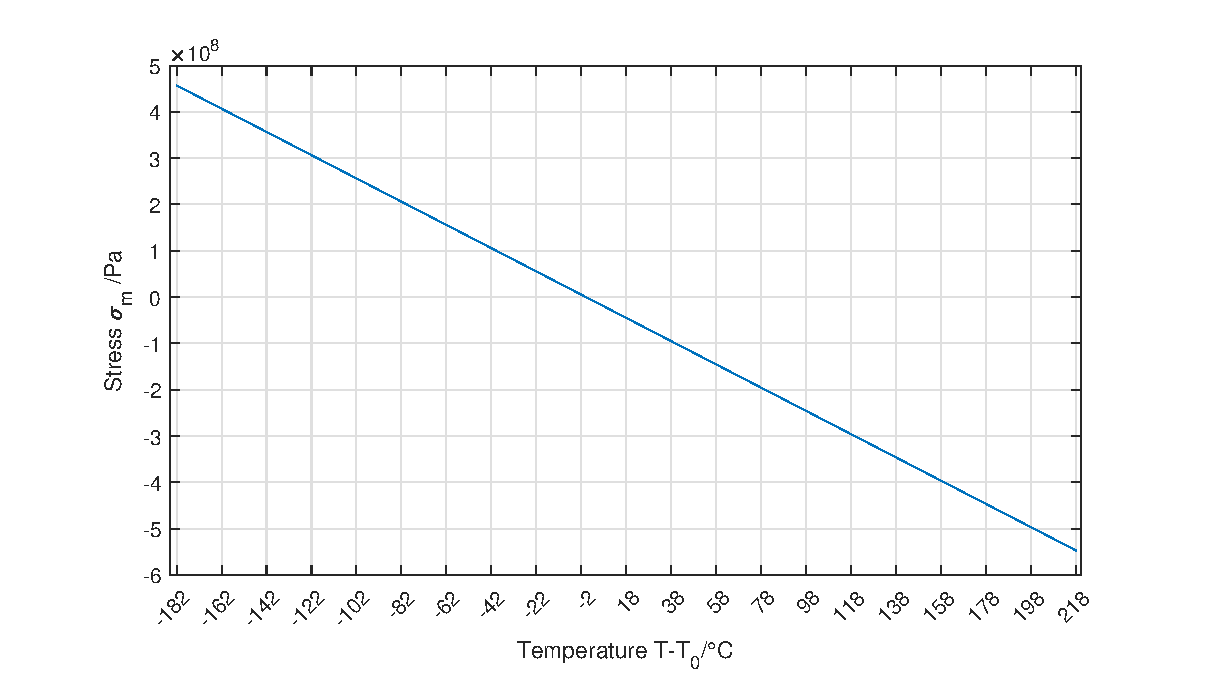
\includegraphics[width = \textwidth]{img/part1ci.eps}
    \caption{Plot of $\sigma_m$ in 3D pipe.}
    \label{part1cSimResults}
\end{figure}
\begin{figure}[H]
    \centering
    \includegraphics[width=\textwidth]{img/part1c-neg160-2.png}
    \caption{3D pipe at time-step 1, \SI{-160}{\degree C}.}
    \label{part1c2}
\end{figure}%
\subsubsection{Comparison against theoretical result and discussion}
The theoretical result was calculated using \ref{stressxx}. MATLAB was used to plot the results. Figure \ref{part1c3} shows the results from ANSYS and MATLAB plotted on the same graph. The variables used in the equation are shown in Table \ref{part1ciiVars}. The value of $M_{Tz}$ was set to zero in this case, as the bending moment
\begin{equation}
    \sigma_{xx} = -\alpha E \left(T - \bar{T}\right) + \frac{M_{Tz}}{I_y}y\label{stressxx}
\end{equation}
\begin{table}[H]
    \centering
    \begin{tabular}{@{}lll@{}}
        \toprule
        \textbf{Variable} & \textbf{Value}                 & \textbf{Source}        \\
        \midrule
        $\alpha$          & \SI{1.196e-05}{\degree C^{-1}} & ANSYS Engineering Data \\
        $E$               & \SI{2.1e11}{\pascal}           & ANSYS Engineering Data \\
        $\bar{T}$         & \SI{22}{\degree C}             & User-defined           \\
        \bottomrule
    \end{tabular}
    \caption{Values of variables used for theoretical calculation of 3D pipe stress.}
    \label{part1ciiVars}
\end{table}
\begin{figure}[H]
    \centering
    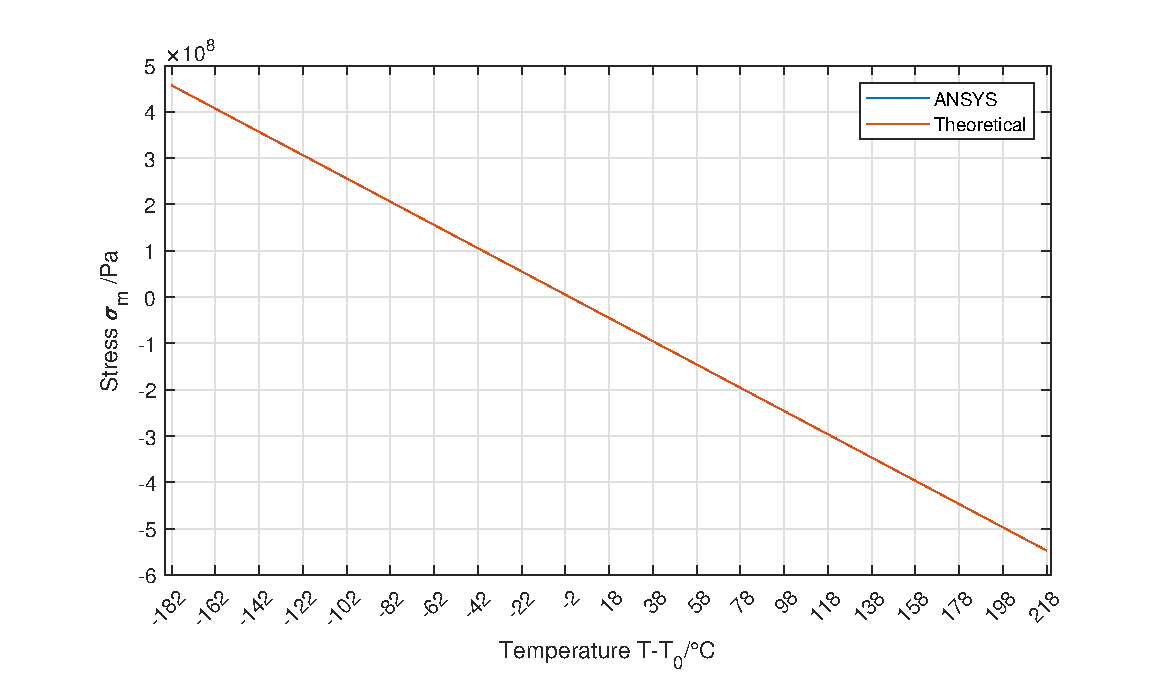
\includegraphics[width = \textwidth]{img/part1cii.eps}
    \caption{Plot of $\sigma_m$ in 3D pipe from ANSYS and theoretical calculation.}
    \label{part1c3}
\end{figure}
The results show a virtually identical stress magnitude. An average percentage of difference of \SI{8.46e-6}{\percent} was calculated for the results.
\subsection{1D pipe ANSYS}\label{part1d}
\url{https://forum.ansys.com/forums/topic/ansys-1d-2d-3d-results-variation/}
\subsubsection{Relationship between maximum stress in temperature range}
\subsubsection{Comparison against theoretical result and discussion}
\subsection{Discussion}
\subsubsection{Difference and similarities between results from \ref{part1b}, \ref{part1c}, \ref{part1d} as pipe slenderness changes}
\subsubsection{Model errors encountered using ANSYS Static Structural model}